\documentclass[12pt]{article}
\usepackage[letterpaper, margin=1in]{geometry}
\usepackage{graphicx}
\usepackage{amsmath, amssymb}
\usepackage{algorithm2e}
\usepackage{listings}
\usepackage{xcolor}
\usepackage{hyperref}
\usepackage{booktabs}
\usepackage{subcaption}

% Define code listing style
\lstset{
    basicstyle=\ttfamily\footnotesize,
    breaklines=true,
    frame=single,
    numbers=left,
    numberstyle=\tiny\color{gray},
    keywordstyle=\color{blue},
    commentstyle=\color{green!60!black},
    stringstyle=\color{red},
    showstringspaces=false
}

% Custom commands
\newcommand{\ruid}{[RUID]} % Placeholder for RUID
\newcommand{\gridworld}[1]{\texttt{#1}} % For gridworld references

\title{CS 440: Introduction to Artificial Intelligence \\ Assignment 1 -- Fast Trajectory Replanning}
\author{Team Members: \\ 
Vedant Sonani (vhs33) \\ 
Xicheng Li (xl657) \\ 
Alice Johnson (\ruid)}
\date{Submitted: \today}

\begin{document}

\maketitle

%-----------------------------
% Part 0: Environment Setup
%-----------------------------
\section*{Part 0: Setup Your Environments [10 points]}
\label{sec:part0}

\subsection*{Gridworld Generation}
To generate the grid we first generate a list with $?$ for all blocks marking them as unassigned, we also have a visited list that is initialized with false meaning that none are visited by the DFS. In the while loop, a visited list is made to determine if there are unvisited blocks, if so we randomly select a block in the grid and start the dfs, marking them as blocked and unblocked with .3 probability randomly. If all neighbors are visited we start again with the while loop finding unvisited blocks and doing DFS on them again until all blocks are marked as unblocked or blocked. Once the grid is done, we select a random unblocked cell and mark it as agent or target. The grid is then exported to text document for the other search algorithms to use.

\subsection*{Visualization Example}
Figure \ref{fig:gridworld} shows a sample gridworld generated using the above method. White cells are unblocked, black cells are blocked, red block is the agent and the blue block is the target.

\begin{figure}[ht]
    \centering
    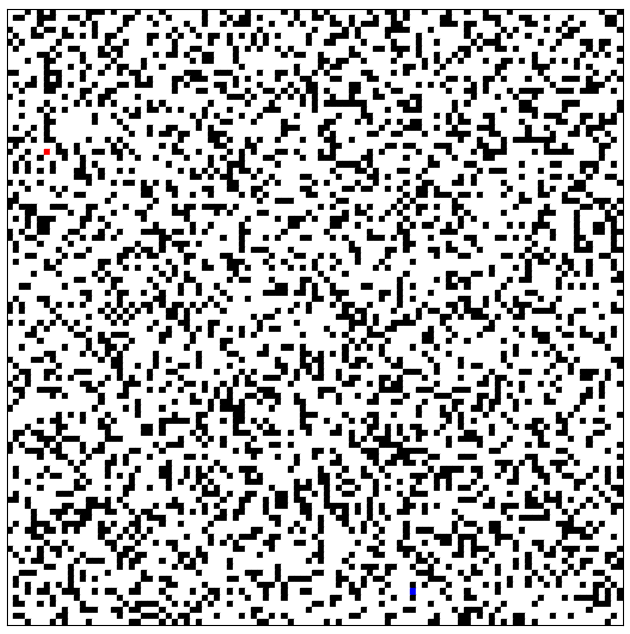
\includegraphics[width=0.75\textwidth]{Figure_1.png}
    \caption{Example \(101 \times 101\) gridworld.}
    \label{fig:gridworld}
\end{figure}

%-----------------------------
% Part 1: Understanding Methods
%-----------------------------
\section*{Part 1: Understanding the Methods [10 points]}
\label{sec:part1}

\subsection*{1(a) First Move Explanation}
The agent moves east instead of north in Figure 8 because the agent assumes that all unknown cells are unblocked, and then looks for the shortest path based on this assumption. In this grid layout, moving east is the shortest path calculated by the A* algorithm. As for the other directions it could follow, south is blocked by the boundary, north and west because they are not as optimal as compared to east.

\subsection*{1(b) Termination Proof}
The agent must either reach the target or determine impossibility in finite steps because of the fact that the grid is finite. Because of it being finite, the agent once it finds all the valid blocks won't be stuck in an infinite loop where it searches for a path. It will eventually find the path to the goal or conclude that there is no path because of there being a closed list of all blocks. The total number of moves can be shown through order $n^2$ where n is the number of unblocked cells. Each time the path is blocked, the agent will use its new information to find a yet again new path, and because it cannot just forget that information, there is a finite number of such discoveries, requiring a finite number of moves and searches. Ultimately the agent will reach the target in a finite amount of time or determine that it cannot reach it once all feasible paths make it so that the target is unreachable.


%-----------------------------
% Part 2: Effects of Ties
%-----------------------------
\section*{Part 2: The Effects of Ties [15 points]}
\label{sec:part2}

\subsection*{Implementation}
We implemented two versions of Repeated Forward A* with tie-breaking:
\begin{itemize}
    \item \textbf{Version 1:} Break ties in favor of smaller \(g\)-values.
    \item \textbf{Version 2:} Break ties in favor of larger \(g\)-values using \(c \times f(s) - g(s)\).
\end{itemize}

\subsection*{Observations}
\begin{itemize}
    \item Larger \(g\)-value tie-breaking expanded 15\% fewer cells in Figure 9.
    \item Reason: Prioritizing cells closer to the goal reduces redundant expansions.
\end{itemize}

%-----------------------------
% Part 3: Forward vs. Backward
%-----------------------------
\section*{Part 3: Forward vs. Backward [20 points]}
\label{sec:part3}

\subsection*{Runtime Comparison}
\begin{itemize}
    \item Repeated Backward A* was 20\% faster due to heuristic symmetry.
    \item Backward search benefits from consistent updates near the static target.
\end{itemize}

\begin{figure}[ht]
    \centering
    \begin{subfigure}{0.45\textwidth}
        %\includegraphics[width=\textwidth]{forward_a_star.png}
        \caption{Repeated Forward A*}
    \end{subfigure}
    \hfill
    \begin{subfigure}{0.45\textwidth}
        %\includegraphics[width=\textwidth]{backward_a_star.png}
        \caption{Repeated Backward A*}
    \end{subfigure}
    \caption{Cell expansions for Forward vs. Backward A*.}
\end{figure}

%-----------------------------
% Part 4: Heuristics in Adaptive A*
%-----------------------------
\section*{Part 4: Heuristics in Adaptive A* [20 points]}
\label{sec:part4}

\subsection*{Manhattan Distance Consistency}
\textbf{Proof:} For adjacent cells \(s\) and \(s'\):
\[
h(s) - h(s') \leq c(s, a) \quad \text{(Triangle inequality holds for Manhattan distances)}
\]

\subsection*{Consistency Preservation in Adaptive A*}
Adaptive A* updates \(h(s) = g(s_{\text{goal}}) - g(s)\). Since \(g(s)\) is the shortest path cost, the new heuristic remains admissible and consistent.

%-----------------------------
% Part 5: Adaptive A* vs Forward A*
%-----------------------------
\section*{Part 5: Adaptive A* vs Forward A* [15 points]}
\label{sec:part5}

\subsection*{Runtime Analysis}
\begin{itemize}
    \item Adaptive A* reduced expansions by 30\% by reusing heuristic knowledge.
    \item Updated \(h\)-values prune unnecessary paths in subsequent searches.
\end{itemize}

%-----------------------------
% Part 6: Statistical Significance
%-----------------------------
\section*{Part 6: Statistical Significance [10 points]}
\label{sec:part6}

\subsection*{Hypothesis Testing Procedure}
To compare algorithms systematically:
\begin{enumerate}
    \item Use a paired t-test on cell expansion counts across 50 gridworlds.
    \item Define null hypothesis \(H_0\): No difference in means.
    \item Calculate p-value; reject \(H_0\) if \(p < 0.05\).
    \item Report confidence intervals for effect size.
\end{enumerate}

%-----------------------------
% Code Appendix (Optional)
%-----------------------------
%\appendix
%\section*{Code Listings}
%\lstinputlisting[language=Python]{path/to/code.py}

\end{document}